%!TEX root = ../terrainbook.tex

\setchapterpreamble[u]{\margintoc}
\labch{spatialextent}
\graphicspath{{spatialextent/}}

\chapter{Spatial extent of a point cloud}%
\label{chap:spatialextent}


Given a point cloud, one operation that practitioners often need to perform is to define the spatial extent of the dataset.
That is, they need to define the shape of the region that best abstracts or represents the set of points.
As seen in \reffig{fig:examples1} and \reffig{fig:examples1}, this region is often in two dimensions, for example in the case of an aerial lidar datasets we want to know where the ground is (after removing the points on the water), or in the case of the scanning of the façade of a building, we would like to obtain a polygon that represents where the wall is (omitting the windows).

\begin{figure}
  \centering
  \begin{subfigure}[b]{0.51\linewidth}
    \centering
    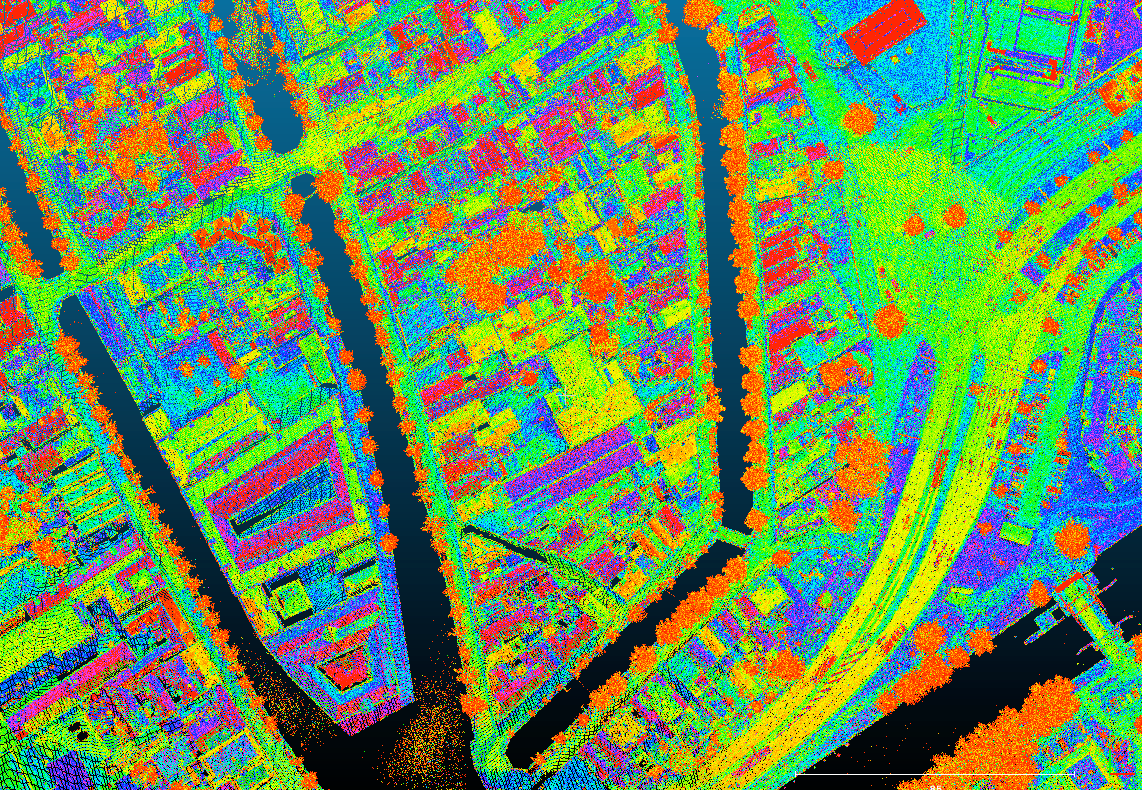
\includegraphics[width=\textwidth]{figs/ahn3-water.png}
    \caption{}
  \end{subfigure}%
  \qquad
  \begin{subfigure}[b]{0.33\linewidth}
    \centering
    \includegraphics[page=2,width=\textwidth]{figs/facade.jpg}
    \caption{}
  \end{subfigure}
\caption{Two point cloud datasets for which we would like to find the spatial extent. \textbf{(a)} An aerial point cloud with several canals (dark colour). \textbf{(b)} A scan of a façade containing several windows.}
\labfig{fig:examples}  
\end{figure}

%

Calculating the spatial extent is useful to calculate the area covered by a dataset, to convert it to other formats (\eg\ raster), or to get an overview of several datasets it is faster to load a few polygons instead of billions of points, etc.

%

The spatial extent is often called by different names, for instance: envelope, hull, concave hull, or footprints.
It is important to notice that the spatial extent is not uniquely defined and that it is a vague concept.
As \reffig{fig:ideas} shows, there are several potential regions for a rather simple set of points, and most of these could be considered `correct' by a human.
\begin{figure}
  \centering
  \begin{subfigure}[b]{0.4\linewidth}
    \centering
    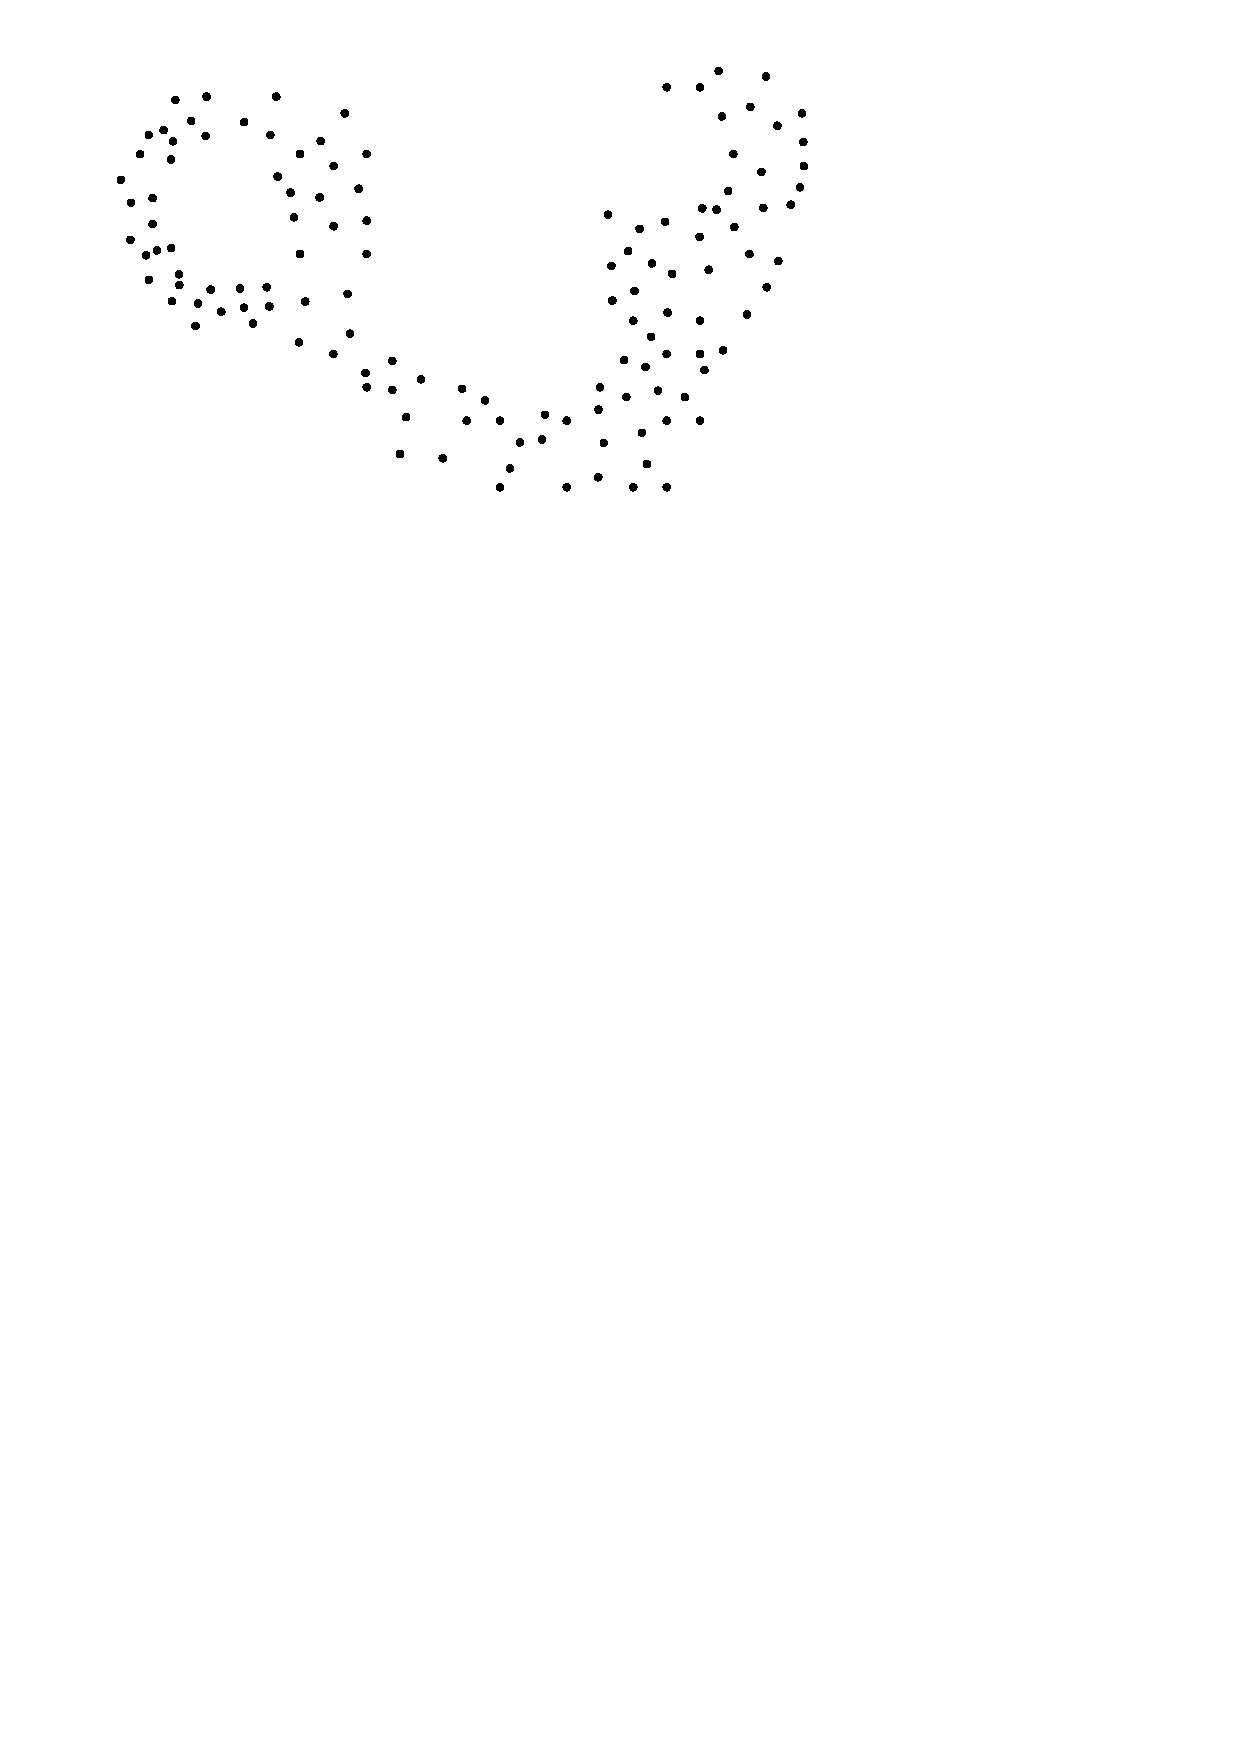
\includegraphics[page=1,width=\textwidth]{figs/idea.pdf}
    \caption{A set of points in $\mathbb{R}^2$}
  \end{subfigure}
  \qquad
  \begin{subfigure}[b]{0.4\linewidth}
    \centering
    \includegraphics[page=2,width=\textwidth]{figs/idea.pdf}
    \caption{Its convex hull}
  \end{subfigure}
  \qquad
  \begin{subfigure}[b]{0.4\linewidth}
    \centering
    \includegraphics[page=3,width=\textwidth]{figs/idea.pdf}
    \caption{A $\chi$-shape}
  \end{subfigure}%
  \qquad
  \begin{subfigure}[b]{0.4\linewidth}
    \centering
    \includegraphics[page=4,width=\textwidth]{figs/idea.pdf}
    \caption{An $\alpha$-shape}
  \end{subfigure}
\caption{Different methods to obtain the spatial extent of a given set of points in the plane.}%
\labfig{fig:ideas}  
\end{figure}

%

In this chapter we present methods that are used in practice to define the spatial extent of a set of points in $\mathbb{R}^2$, which implies that the points in a point cloud are first projected to a two-dimensional plane.



%%%%%%%%%%%%%%%%%%%%
%
\section{Properties of the region}
\label{sec:properties}

\begin{figure*}
  \centering
  \begin{subfigure}[b]{0.2\linewidth}
    \centering
    \includegraphics[page=2,width=\textwidth]{figs/properties.pdf}
    \caption{}
    \labfig{fig:properties:a}
  \end{subfigure}%
  \qquad
  \begin{subfigure}[b]{0.2\linewidth}
    \centering
    \includegraphics[page=4,width=\textwidth]{figs/properties.pdf}
    \caption{}
    \labfig{fig:properties:b}
  \end{subfigure}
  \qquad
  \begin{subfigure}[b]{0.2\linewidth}
    \centering
    \includegraphics[page=5,width=\textwidth]{figs/properties.pdf}
    \caption{}
    \labfig{fig:properties:c}
  \end{subfigure}%
  % \qquad
  % \begin{subfigure}[b]{0.2\linewidth}
  %   \centering
  %   \includegraphics[page=6,width=\textwidth]{figs/properties.pdf}
  %   \caption{}
  %  \label{g:properties:a}
  % \end{subfigure}
  \qquad
  \begin{subfigure}[b]{0.2\linewidth}
    \centering
    \includegraphics[page=3,width=\textwidth]{figs/properties.pdf}
    \caption{}
    \labfig{fig:properties:d}
  \end{subfigure}
\caption{Different properties for the spatial extent}%
\labfig{fig:properties}  
\end{figure*}

Let $S$ be a set of points in $\mathbb{R}^2$, and $R(S)$ the region that characterise the spatial extent of $S$.
The region is potentially formed by a set of polygons (if $S$ forms two distinct clusters for instance), and in practice most algorithms will compute a linear approximation of $R(S)$, so the polygons will have straight edges as boundaries.

To evaluate the different algorithms to create R($S$), we list here different properties that one must consider when defining the spatial extent of a set of points.
\begin{description}
  \item[P1.] \textbf{\emph{Regular} polygons?} Are polygons allowed to have dangling parts (lines), such as the one in \reffig{fig:properties:b}
  % \item[P2.] \textbf{Are points allowed to be on the boundary of the region?} All of the regions in \reffig{fig:properties} (except d) have points on the boundary of $R(S)$.
  \item[P2.] \textbf{All points part of the region?} Can outliers be ignored? Or do they have to be part of the region? In \reffig{fig:properties:a} and \reffig{fig:properties:b} they are all part of the region, in \reffig{fig:properties:c} and \reffig{fig:properties:d} one outlier is not.
%   (if we consider that $S$ represents the letter ``b'').
  \item[P3.] \textbf{Region is one connected component?} Or are more components allowed? In \reffig{fig:properties:a}--\reffig{fig:properties:c} there is one component, but \reffig{fig:properties:d} has two.
  \item[P4.] \textbf{Are holes allowed in a polygon?} Polygons in \reffig{fig:properties:a}--\subref{fig:properties:c} have only an exterior boundary, while in \reffig{fig:properties:d} one polygon has an interior boundary too (a hole).
  \item[P5.] \textbf{Computational efficiency} What is the time complexity of the algorithm, and does it require large and complex auxiliary data structures?
\end{description}



%%%%%%%%%%%%%%%%%%%%
%
\section{Convex hull}

As explained in Section~\ref{sec:convexhull}, given $S$, a set of points in $\mathbb{R}^2$, its convex hull, which we denote conv($S$), is the minimal convex set containing $S$.
Two examples of convex hulls are in Figures~\ref{fig:ideas}b and~\ref{fig:properties}a.

%

For a given set of points, the convex hull is uniquely defined and does not require any parameters (unlike the other methods listed below).
It is also relatively easy to compute: it can be extracted from the Delaunay triangulation, or compute directly using a specialised algorithm.
For example, using the well-known \emph{gift wrapping algorithm}, shown in \reffig{fig:giftwrapping}.
\begin{marginfigure}
  \centering
  \begin{subfigure}[b]{\linewidth}
    \centering
    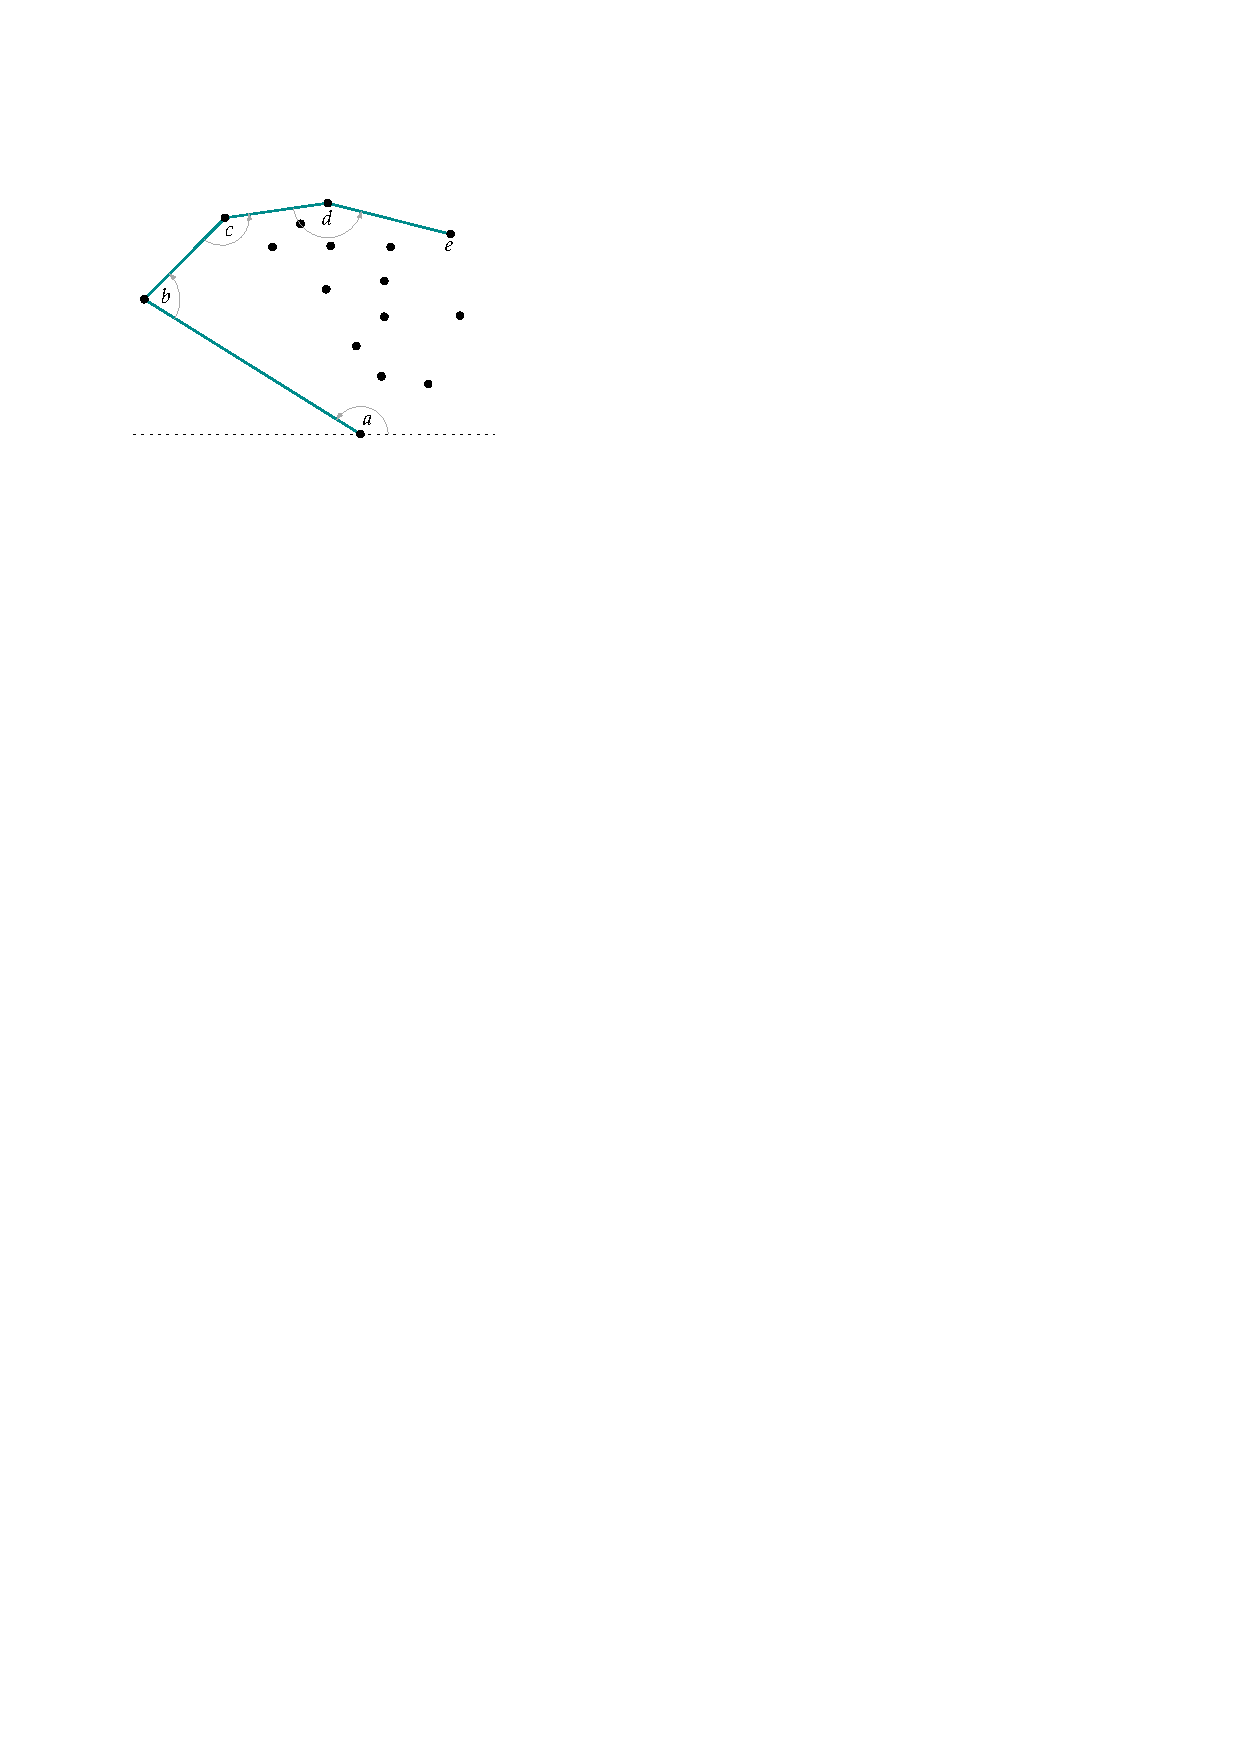
\includegraphics[page=1,width=\textwidth]{figs/giftwrapping.pdf}
    \caption{}
  \end{subfigure}
  \qquad
  \begin{subfigure}[b]{\linewidth}
    \centering
    \includegraphics[page=2,width=\textwidth]{figs/giftwrapping.pdf}
    \caption{}
  \end{subfigure}
  \caption{\textbf{(a)} First four steps of the gift wrapping algorithm to compute the convex hull. \textbf{(b)} The resulting convex hull.}%
\labfig{fig:giftwrapping}
\end{marginfigure}
It begins with a point that is guaranteed to be on conv($S$) (we can take an `extreme', such as $a$ in \reffig{fig:giftwrapping} because it is the point with the lowest $y$-coordinate), and then picks the point in $S$ (omitting the ones already on conv($S$)) for which the polar angle between the horizontal line and that point (at $a$) is the smallest ($b$ in this case), and adds it to conv($S$).
Then for $b$, the polar angle is calculated from the line $ab$; and the algorithm continues this way until $a$ is visited again.

If $S$ has $n$ points and conv($S$) is formed of $h$ points, then the gift wrapping algorithm has a time complexity of $\mathcal{O}(n \, h)$; each of the $h$ points are tested against all $n$ points in $S$.
However, there exist more efficient algorithm that have a time complexity of $\mathcal{O}(n \log n)$.

%
Properties convex hull:
\\
\begin{tabular}{@{}ll@{}}
\toprule
  P1. & The sole polygon is guaranteed to be regular (and convex).  \\  
  % P2. & A subset of $S$, or all of them, forms the region. \\ 
  P2. & All points are on or inside the region. \\ 
  P3. & One component.  \\ 
  P4. & No holes in the region.  \\  
  P5. & $\mathcal{O}(n \log n)$  \\  
\bottomrule
\end{tabular}



%%%%%%%%%%%%%%%%%%%%
%
\section{Moving arm}

\begin{marginfigure}
  \centering
  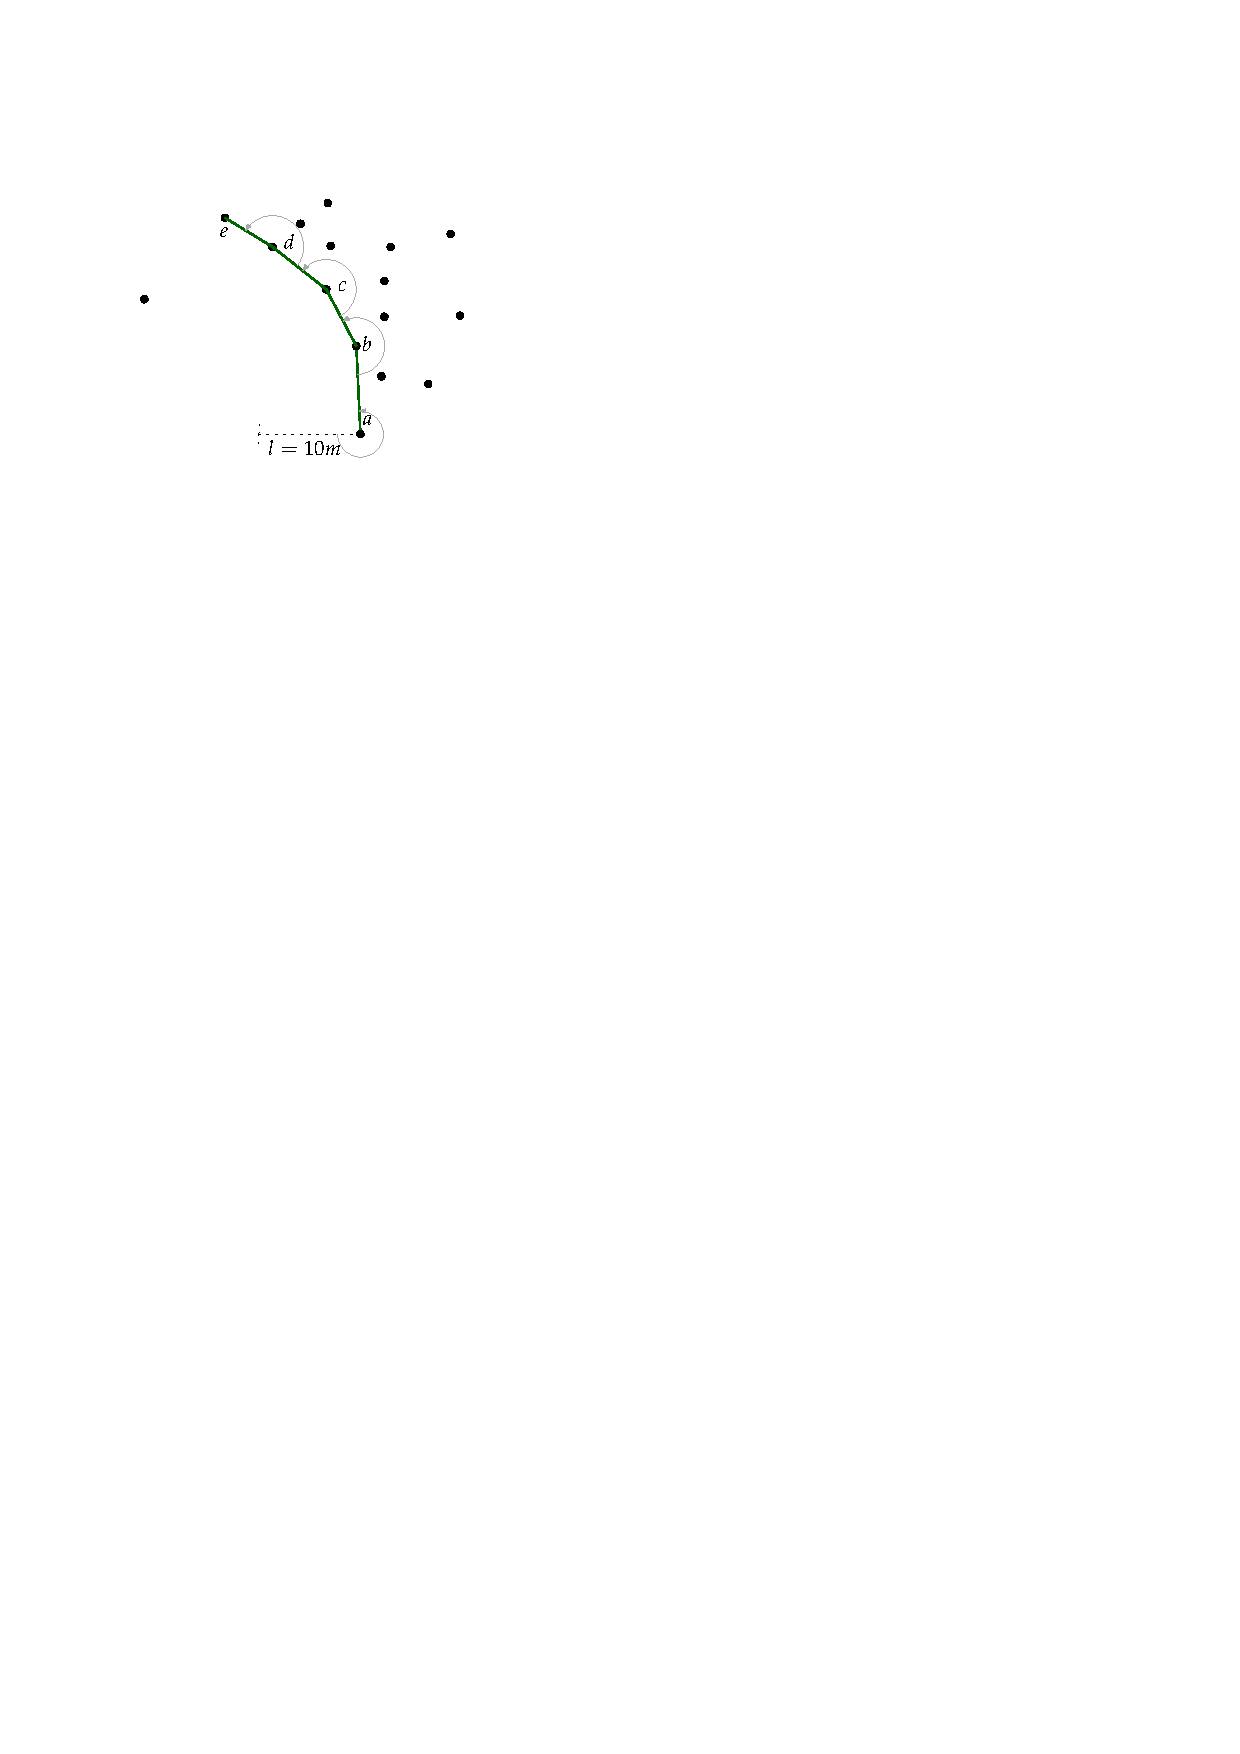
\includegraphics[page=1,width=\textwidth]{figs/movingarm.pdf}
  \caption{First four steps of the \emph{moving arm algorithm} (with a lenght $l$) to compute the spatial extent.}%
\labfig{fig:movingarm:1}
\end{marginfigure}

\begin{marginfigure}
  \centering
  \includegraphics[page=2,width=\textwidth]{figs/movingarm.pdf}
  \caption{First four steps of the \emph{moving arm algorithm} (with a \emph{knn} where $k=3$) to compute the spatial extent.}%
\labfig{fig:movingarm:2}
\end{marginfigure}

\begin{marginfigure}
  \centering
  \includegraphics[page=3,width=.9\textwidth]{figs/movingarm.pdf}
  \caption{The resulting region for the moving arm, it is concave. Observe that 1 point from $S$ (highlighted in red) is not part of the region.}%
\labfig{fig:movingarm:3}
\end{marginfigure}

\paragraph{Arm of length $l$.} 
The moving arm is a generalisation of the gift wrapping algorithm where the infinite line, used to calculate the polar angles, is replaced by a line segment of a given length $l$ (the ``moving arm'').
This means that, unlike the original gift wrapping algorithm, only a subset of the points in $S$ are considered at each step.
This also means that potentially the result is a polygon that is non-convex.
\reffig{fig:movingarm:1} shows the first few steps for a given $l$, and it can be observed that 1 point is not part of the final region.
Observe also that if $l$ had been larger then conv($S$) could have been obtained.


%

\paragraph{Adaptative arm with \emph{knn}.} 
There exists a variation of this algorithm where the length of the moving arm is adaptive at each step; the $k$ nearest neighbours (knn) of a given point $p$ are used to determine it (see Section~\ref{sec:kdtree}).
As can be seen in \reffig{fig:movingarm:2}, the largest polar angle, as used for gift wrapping algorithm, is used to select the point at each step.

%

\paragraph{No guarantee that it will work.} 
Both versions of the algorithm will work in most cases, but there is no guarantee that they will for all inputs.
\reffig{fig:movingarm_kdd} shows a concrete example.
\begin{marginfigure}
  \centering
  \begin{subfigure}[b]{.9\linewidth}
    \centering
    \includegraphics[page=4,width=\textwidth]{figs/movingarm.pdf}
    \caption{}
  \end{subfigure}
  \qquad
  \begin{subfigure}[b]{.9\linewidth}
    \centering
    \includegraphics[page=5,width=\textwidth]{figs/movingarm.pdf}
    \caption{}
  \end{subfigure}
\caption{Moving arm with \emph{kdd} when $k=4$. \textbf{(a)} When the point $e$ is being processed, $f$ is the next one chosen. \textbf{(b)} From $f$, no other points can be chosen since the resulting region would be self-intersecting.}%
\labfig{fig:movingarm_kdd}
\end{marginfigure}
In this case, a solution to this problem would be to either choose another $k$, or to rotate counter-clockwise instead of clockwise, which will in practice yield different results.


%
\paragraph{Different clusters?} 
One drawback of the moving arm method is that only one polygon is obtained as a region.
If $S$ forms different clusters (see for instance \reffig{fig:clusters}, then only the cluster that is the `lowest' will be output for the region (since the lowest point is picked as a starting point).
\begin{marginfigure}
  \includegraphics[page=2,width=.9\textwidth]{figs/clusters.pdf}
  \caption{$S$ has two distinct clusters. In green the typical output if $S$ processed as a single cluster with a moving arm algorithm.}%
\labfig{fig:clusters}
\end{marginfigure}
Notice that this can also be useful to discard unwanted outliers (unless the lowest point is an outlier).
In practice, the problem of several clusters can be solved by preprocessing the input points with a clustering algorithm (in the case of \reffig{fig:clusters} two clusters should be detected) and then each cluster is processed separately.

%

The worst case time complexity is the same as for the gift wrapping algorithm: $\mathcal{O}(n \, h)$.
If a $k$d-tree is used, this stays the same but in practice will be sped up as the subset of $S$ tested will be smaller. 
Each query in a $k$d-tree takes $\mathcal{O}(\log n)$ on average, but we need to store an auxiliary structure that takes $\mathcal{O}(n)$ storage.

Properties moving arm:
\\
\begin{tabular}{@{}ll@{}}
\toprule
  P1. & The sole polygon could be degenerate (self-intersection).  \\  
  P2. & Outliers can be discarded (except if it is the lowest point) \\
  P3. & One component.  \\ 
  P4. & No holes in the region.  \\  
  P5. & $\mathcal{O}(n \, h)$  \\  
\bottomrule
\end{tabular}


\newpage
%%%%%%%%%%%%%%%%%%%%
%
\section{$\chi$-shape}

\begin{marginfigure}
  \centering
  \begin{subfigure}[b]{0.6\linewidth}
    \centering
    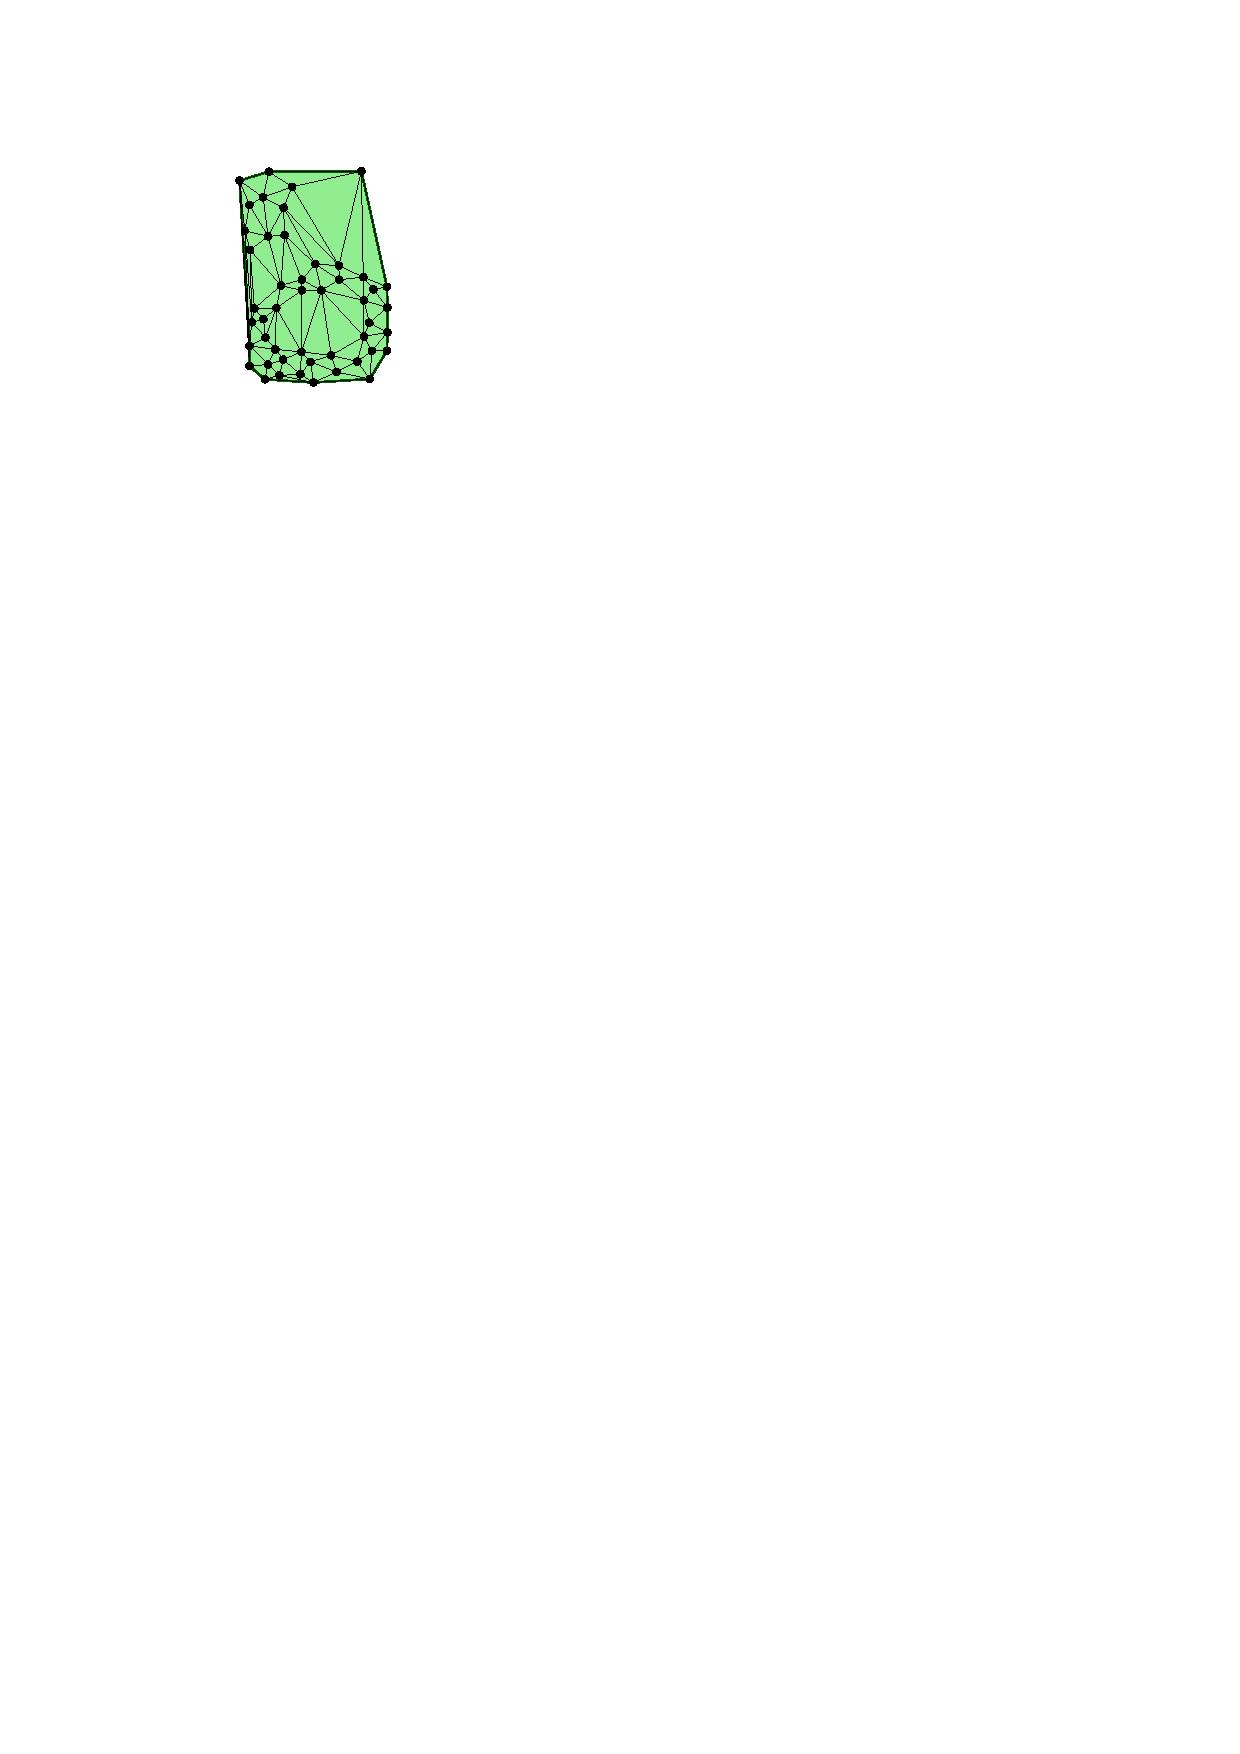
\includegraphics[page=1,width=\textwidth]{figs/chishape.pdf}
    \caption{}
  \end{subfigure}
  \qquad 
  \begin{subfigure}[b]{0.6\linewidth}
    \centering
    \includegraphics[page=2,width=\textwidth]{figs/chishape.pdf}
    \caption{}
  \end{subfigure}
  \qquad 
  \begin{subfigure}[b]{0.6\linewidth}
    \centering
    \includegraphics[page=3,width=\textwidth]{figs/chishape.pdf}
    \caption{}
  \end{subfigure}
\caption{$\chi$-shape examples. \textbf{(a)} $S$, its DT, and its envelope (cons($S$)). \textbf{(b)} After some edges have been removed. \textbf{(c)} The final result for a given threshold. Observe that neither of the red edges can be removed because a self-intersection would be created}%
\labfig{fig:chishape}
\end{marginfigure}

The $\chi$-shape is based on first constructing the Delaunay triangulation (DT) of $S$, and then removing iteratively the longest edge forming the envelop (at first this envelop is conv($S$)) until no edge is longer than a given threshold $l$.
The idea is to construct one polygon that is potentially non-convex, and that contains all the points in $S$.
Before removing an edge, we must verify that it will not introduce a topological issue in the envelop, that is that the envelop will not contain a self-intersection (see \reffig{fig:chishape}c, the dangling edge is there twice, once in each direction). 

%

A DT can be constructed in $\mathcal{O}(n log n)$.
The number of edges in a DT of $n$ points is roughly $3n$ (thus $\mathcal{O}(n)$), and since verifying the topological constraint can be done locally (previous and next edge) the overall time complexity is $\mathcal{O}(n \log n)$

Properties $\chi$-shape:
\\
\begin{tabular}{@{}ll@{}}
\toprule
  P1. & The sole polygon is guaranteed to be regular.  \\  
  % P2. & A subset of $S$, or all of them, forms the region. \\ 
  P2. & All points are part of the region \\ 
  P3. & One component.  \\ 
  P4. & No holes in the region.  \\  
  P5. & $\mathcal{O}(n log n)$  \\  
\bottomrule
\end{tabular}


%%%%%%%%%%%%%%%%%%%%
%
\section{$\alpha$-shape}

The $\alpha$-shape is conceptually a generalisation of the convex hull of a set $S$ of points.
% The $\alpha$-shape has stronger mathematical foundations then the alternatives mentioned above, and conceptually, it is a generalisation of the convex hull of a set $S$ of points.
% While the concepts are valid in any dimension, let us explain it here for the two-dimensional case.

%

It is best understood with the following analogy.
First imagine that $\mathbb{R}^2$ is filled with Styrofoam and that the points in $S$ are made of hard material.
Now imagine that you have a carving tool which is a circle of radius $\alpha$, and that this tool can be used anywhere from any direction (it is `omnipresent'), and that it is only stopped by the points.
The result after carving, called the $\alpha$-hull, is one or more pieces of Styrofoam.
If we straighten the circular edges, then we obtain the $\alpha$-shape.
See \reffig{fig:alphashape} for an example.
\begin{figure*}
  \centering
  \begin{subfigure}[b]{0.15\linewidth}
    \centering
    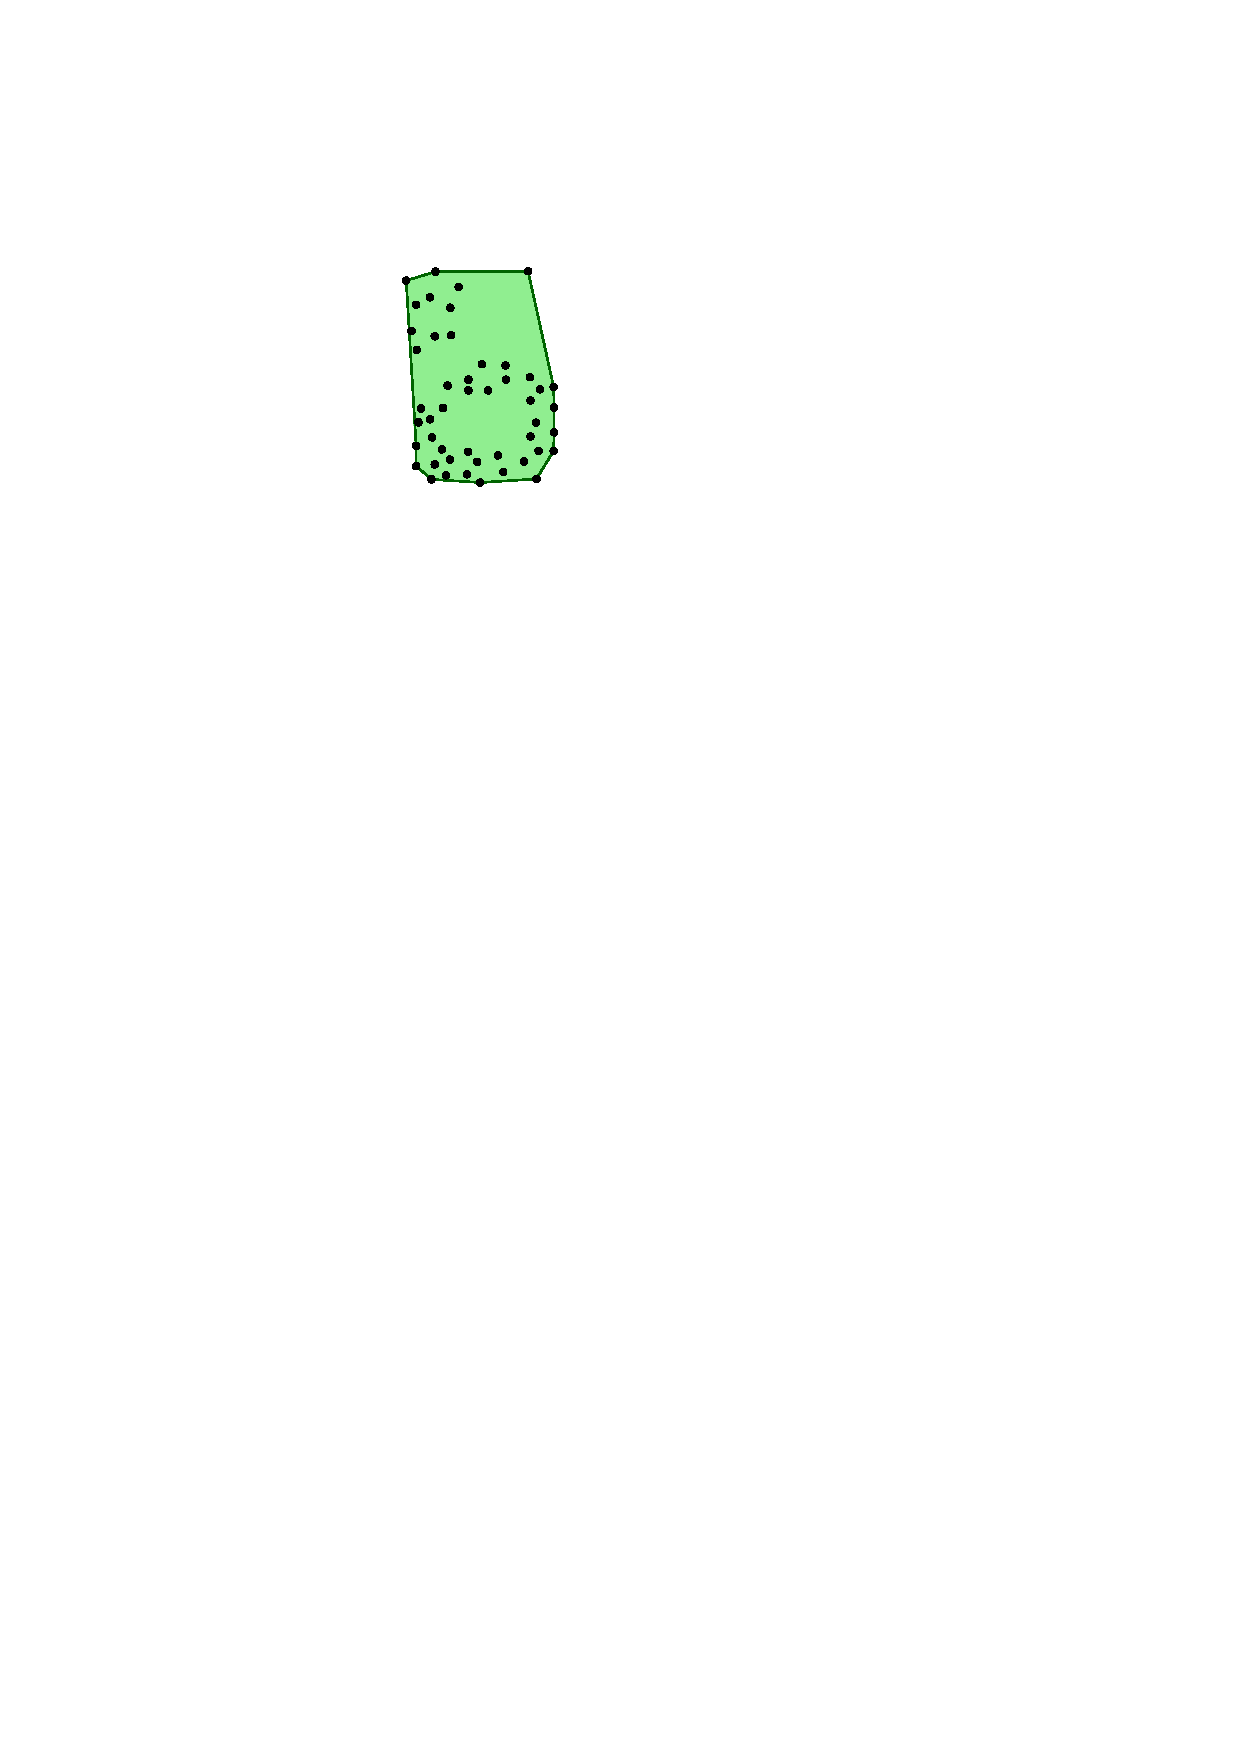
\includegraphics[page=1,width=\textwidth]{figs/alphashape.pdf}
    % \caption{}\labfig{fig:aplhashape:a}
  \end{subfigure}
  \qquad 
  \begin{subfigure}[b]{0.15\linewidth}
    \centering
    \includegraphics[page=2,width=\textwidth]{figs/alphashape.pdf}
    % \caption{}\labfig{fig:aplhashape:b}
  \end{subfigure}
  \qquad 
  \begin{subfigure}[b]{0.15\linewidth}
    \centering
    \includegraphics[page=3,width=\textwidth]{figs/alphashape.pdf}
    % \caption{}\labfig{fig:aplhashape:c}
  \end{subfigure}
  \qquad 
  \begin{subfigure}[b]{0.15\linewidth}
    \centering
    \includegraphics[page=4,width=\textwidth]{figs/alphashape.pdf}
    % \caption{}\labfig{fig:aplhashape:d}
  \end{subfigure}
  \qquad 
  \begin{subfigure}[b]{0.15\linewidth}
    \centering
    \includegraphics[page=5,width=\textwidth]{figs/alphashape.pdf}
    % \caption{}\labfig{fig:aplhashape:e}
  \end{subfigure}
\caption{Five $\alpha$-shape for the same set of points, with decreasing $\alpha$ values from left to right.}%
\labfig{fig:alphashape}
\end{figure*}


%

Now let $\alpha$ be a real number with $0 \leq \alpha \leq \infty$.
If $\alpha = \infty$, then the $\alpha$-shape is conv($S$) because you will not be able to carve inside conv($S$).
As $\alpha$ decreases, the $\alpha$-shape shrinks and cavities can appear, and different components can be created.
If $\alpha = 0$ then the $\alpha$-shape is $S$ (which is a valid $\alpha$-shape).

%

The $\alpha$-shape is not a polygon or a region, but a complex formed of $k$-simplices, where $0 \leq k \leq 2$.
Furthermore, it is a subcomplex of the Delaunay triangulation (DT) of $S$.
That is, the easiest method to construct an $\alpha$-shape is by first constructing DT($S$), and then removing all edges that are shorter then $2\alpha$.

In practice, all the $\alpha$-shapes of $S$ (for different values of $\alpha$) can be calculated and discretised since we know that $\alpha$ will range from the shortest edge to the longest.
For each $k$-simplex, we can thus assign a range where it will be present.
Implementations of the $\alpha$-shape will often offer to compute automatically an $\alpha$ such that the complex obtained is for instance connected and contains only one polygon.

%

A DT can be constructed in $\mathcal{O}(n log n)$ time, and the algorithm only requires to visit once each of the $\mathcal{O}(n)$ triangles, thus the time complexity is $\mathcal{O}(n log n)$.

%

Properties $\alpha$-shape:
\\
\begin{tabular}{@{}ll@{}}
\toprule
  P1. & A complex of $k$-simplices.  \\  
  % P2. & A subset of $S$, or all of them, are on the boundary of the region. \\ 
  P2. & Some points can be omitted. \\ 
  P3. & Several components possible.  \\ 
  P4. & Regions can contain holes.  \\  
  P5. & $\mathcal{O}(n log n)$  \\ 
\bottomrule
\end{tabular}



%%%%%%%%%%%%%%%%%%%%
%
\section{Notes \& comments}

The properties listed in Section~\ref{sec:properties} are taken, and slightly adapted, from \citet{Galton06}. 

The \emph{quickhull} algorithm is the most known and used convex hull algorithm, and it is valid in any dimensions. See \citet{Barber96} for the details, and \url{http://www.qhull.org/} for implementations.

The gift wrapping algorithm to compute the convex hull of a set of points in $\mathbb{R}^2$ is from \citet{Jarvis73}.

The moving arm with a length is presented and described in \citet{Galton06}, and the adaptative one in \citet{Moreira07}.
In both papers, the authors describe different strategies to make the algorithm work for all input, but these do not have any warranty to output a simple polygon.

The $\chi$-shape was introduced in \citet{Duckham08}.

The explanation of the $\alpha$-shape is taken from \citet{Edelsbrunner94} and from the CGAL documentation\sidenote{\url{https://doc.cgal.org/latest/Alpha_shapes_2/index.html}}.

% TODO: add that stuff?
% https://en.wikipedia.org/wiki/DBSCAN
% https://en.wikipedia.org/wiki/Gift_wrapping_algorithm#/media/File:Animation_depicting_the_gift_wrapping_algorithm.gif

%%%%%%%%%%%%%%%%%%%%
%
\section{Exercises}

\begin{enumerate}
  \item Given a DT($S$), how to extract conv($S$)?
  \item What are the disadvantages of the $\chi$-shape compared with the $\alpha$-shape?
  \item If the parameter $l$ for the $\chi$-shape is equal to the $\alpha$ parameter for an $\alpha$-shape, will the resulting shapes be the same?
  \item Given an $\alpha$-shape of $S$, how to calculate how many components are part of it? 
  \item Draw what would happen if one of the 2 edges was removed in \reffig{fig:chishape}c.
  \item What is the influence of $k$ for the moving arm algorithm (with a \emph{kdd})? Will a higher $k$ create a larger or smaller region in general?
\end{enumerate}


